\chapter{Introduction}

\section{Purpose}

\section{Motivation}

\subsection{Why build web applications for Systems Biology?}

\subsubsection{The challenge of software deployment and adoption}

\subsubsection{Scientific reproducibility}

\subsubsection{Scalable applications}

\section{A Brief History of Web Applications}
\autocite{w3c2014history}
\autocite{berners2014design}
\begin{itemize}
  \item 1980: Tim Berners-Lee, at CERN, made ENQUIRE a system to use and share documents
  \item 1991: HTML publicly released
  \item 1995: JavaScript written in 10 days by Brendan Eich to be released with Netscape Navigator 2.0
  \item 1996: CSS, 
  \item 1997: ECMAScript 1
  \item 1998: ECMAScript 2
  \item 1999: ECMAScript 3
  \item 2006: jQuery released
  \item 2008: JavaScript the Good Parts 176 pages, JavaScript the Definitive Guide 1100 pages
  \item 2009: Node.js, Angular.js, ECMAScript 5
  \item 2010-today: Backbone, Knockout.js, Ember, Handlebars.js, etc\ldots

\end{itemize}

\subsection{DOM}

\begin{figure}
  \centering
  \includegraphics[width=\textwidth,page=3]{images/Figures.pdf}
  \caption{How JQuery and Angular scale for complex JavaScript Web Applications.}
  \label{Figure:}
\end{figure}

\subsection{HTML5}
\label{sec:html5}

\subsection{Single Page Web Applications}

\begin{figure}
  \centering
  \includegraphics[width=\textwidth,page=3]{images/Figures.pdf}
  \caption{How JQuery and Angular scale for complex JavaScript Web Applications.}
  \label{Figure:jquery-vs-angular}
\end{figure}

declarative programming should be used for building user interfaces and wiring software components, while imperative programming is excellent for expressing business logic


Decouple DOM manipulation from application logic. This improves the testability of the code. Regard application testing as equal in importance to application writing. Testing difficulty is dramatically affected by the way the code is structured.
Decouple the client side of an application from the server side. This allows development work to progress in parallel, and allows for reuse of both sides.
Guide developers through the entire journey of building an application: from designing the UI, through writing the business logic, to testing.
Angular follows the MVC pattern of software engineering and encourages loose coupling between presentation, data, and logic components. Using dependency injection, Angular brings traditional server-side services, such as view-dependent controllers, to client-side web applications. Consequently, much of the burden on the backend is reduced, leading to much lighter web applications.


\section{Specific Results}
\subsection{Aim 1 - Chapter~\ref{chap:graphene}: Produce a web library for building interactive and graphical applications}
\subsection{Aim 2 - Chapters~\ref{chap:tidal},~\ref{chap:redox}: Integrate Graphene into new and existing applications}
\subsection{Aim 3 - Chapters~\ref{chap:carbon},~\ref{chap:engine}: Build server-side architecture for modeling applications}

